%\lhead{\sffamily  {\small Dark Energy}}
\lhead{{\small LSST undergraduate internships at Fermilab}}

\section{LSST Data Science Internships at Fermilab}

% For student internship proposals, 
% describe the student or selection process, mentoring strategies, and a summary of the 
% existing internship program if the proposal is to augment that. 

 
We propose to build on last year's successful research mentorship program for undergraduates at the Center for Particle Astrophysics at Fermilab.
Students will participate in data-driven LSST science projects, implementing data science tools (e.g, statistics, machine learning, and high-performance computing) and engaging in training and tutorials on these tools.
Our capabilities in image processing, cosmological modeling, and machine learning combine for a uniquely powerful
data science experience for students and a research advancement for mentors.
Will also implement regular training for science communication, and inculcate best practices in software development.


The 7$^{th}$ floor at Fermilab's Wilson Hall is the home to a 
group of experimental astrophysicists that once helped build and operate
the revolutionary Sloan Digital Sky Survey, helped build and operate
the evolutionary Dark Energy Survey, and will soon be helping to operate 
the revolutionary Large Synoptic Survey Telescope. Cosmic surveys are
what the group was founded to do in 1992 and what we've been doing for 25 years.

% The culture here is interesting: for example, the postdocs do not work for
% a supervisor, they are their own independent scientists. Often our job as 
% staffers here at the Lab is to support the postdocs in their 
% ambitious scientific pursuits. The postdocs 
% often produce astounding results- such as Alex Drilca-Wagner's dwarf galaxy searches,
% which  enabled new limits on dark matter. Our current set of postdocs 
% came to the 7th floor to help us extract science from the DES data stream,
% but each are trying to create something new, something of their own or 
% something jointly with a colleague. Now they are looking to the future,
% looking to perform exciting science  inside the DESC science collaboration.
% These postdocs set our science goals: cluster cosmology, dark matter via
% dwarf galaxy studies, strong lensing, machine learning.

The culture here is driven by our outstanding postdocs and mission to support
world-class cosmology experiments. A strong strand in this culture is mentoring
junior scientists, both  as visitors from collaboration institutions and as participants
in various summer programs.
During the summer the population on the 7th floor more than doubles.
Fermilab's Summer Interns in Science and Technology program (SIST),
DOE's Science Undergraduate Laboratory Interns (SULI), and the University of
Chicago's Metcalf Intern provides undergraduate students. 
Fermilab's TARGET program brings in the best high school 
students from the Chicagoland area for a summer, 
and our relationship with Illinois Math and Science Academy provides
certain high school students with a longer term summer program here.
This coming year two graduate students, one from University of Chicago and the
other from the Ohio University, will study here on the DOE Office of Science
Graduate Student Research Program.

Last year the LSSTC Enabling Science grant allowed us to bring in
4 undergraduate interns and 1 lab manager/intern to pursue LSST
cosmology and graviational wave science. We pulled from a wide geographic base:
two University of Chicago students, one Grinnell College students, 
one (for the second summer) from Macalester Collge, and
one from the University of West Virgina. They joined with 7th floor SIST, SULI,
and Metcalf interns and a team visiting from Brandeis University to form
a mentoring laboratory of 3 postdocs, 2 graduate students, 11 undergraduates, and 4
high school students,
supported by 3 senior scientists. The lab manager model worked well for us- this
being the idea that a more experienced student is brought on to help the summer interns
learn how to do the simple things (at Fermilab the exemplar is learning to print)
without having to engage postdocs or senior scientists. Their time is more valuably
spent mentoring the students on the science.

For the second summer in a row,
the experiment of aiming to have the students learn as much from each other as from
the more senior scientists was encouraging.
Peer groups learn from each other,
and differences in experience represent chances to teach: high school
students learn readily from undergraduates, and undergraduates learn
by leading high school students. 
They used Git to share code, sat in each other's offices to work problems, and
exchanged plots to prepare posters, talks, and reports. 
They self-reported a fantastic experience: each with their strengths,
they felt part of something greater, part of a team building something 
for science. That is, they felt part of the large collaboration experience.
We believe we should build on this.

This summer we will bring a machine learning perspective to last summers
data science endeavors. 

\newpage

We are active in the Dark Energy Science Collaboration and its dark matter component.
We will aim the students at studying the DC2 catalogs. We would ask
the interns to re-create a famous plot in astrophysics and cosmology using
the DC2 catalogs, the CosmoSIS cosmological modeling program,
DESC Jupyter notebooks, Github, and teamwork. Once they have done so,
we ask them to make an improvement. That simple, and that hard.

The actual science we have them do is secondary: perhaps it is the
halo mass function, perhaps it is the galaxy-galaxy correlation function.
All of these are new to undergraduates, and by doing the classics they
become ready to do things new.

We will ask them to ramp up on a machine learning algorithm and
to learn how to apply it in the context of their problem.

We choosee to do this
as we intend to prepare the students to become active scientists
with LSST/DESC science products and there the learning curve is greater.
The reason to try this approach is in the students: where they go next.
Of last year's LSSTC interns, two are applying for graduate school,
one is taking a year off before applying to graduate school, and one
will be a senior in the fall.
Our aim is to build a summer laboratory 
that prepares junior scientists to thrive in the LSST era: there
are several paths to do this. 

To summarize, we  propose to leverage off of the tradition 
of mentoring at Fermilab by
bringing on two undergraduate interns from this funding
and several more from existing Fermilab intern programs.
The interns will form a lab around a more experience
lab manager, and will explore the science
of combining DC2 science analysis with CosmoSIS modeling
under the supervision of experienced cosmic
frontier scientists, a model that was shown to work
well last year. Many of these  undergraduates will
form the candidate graduate student classes in years to come.

\begin{figure}
  \centering
    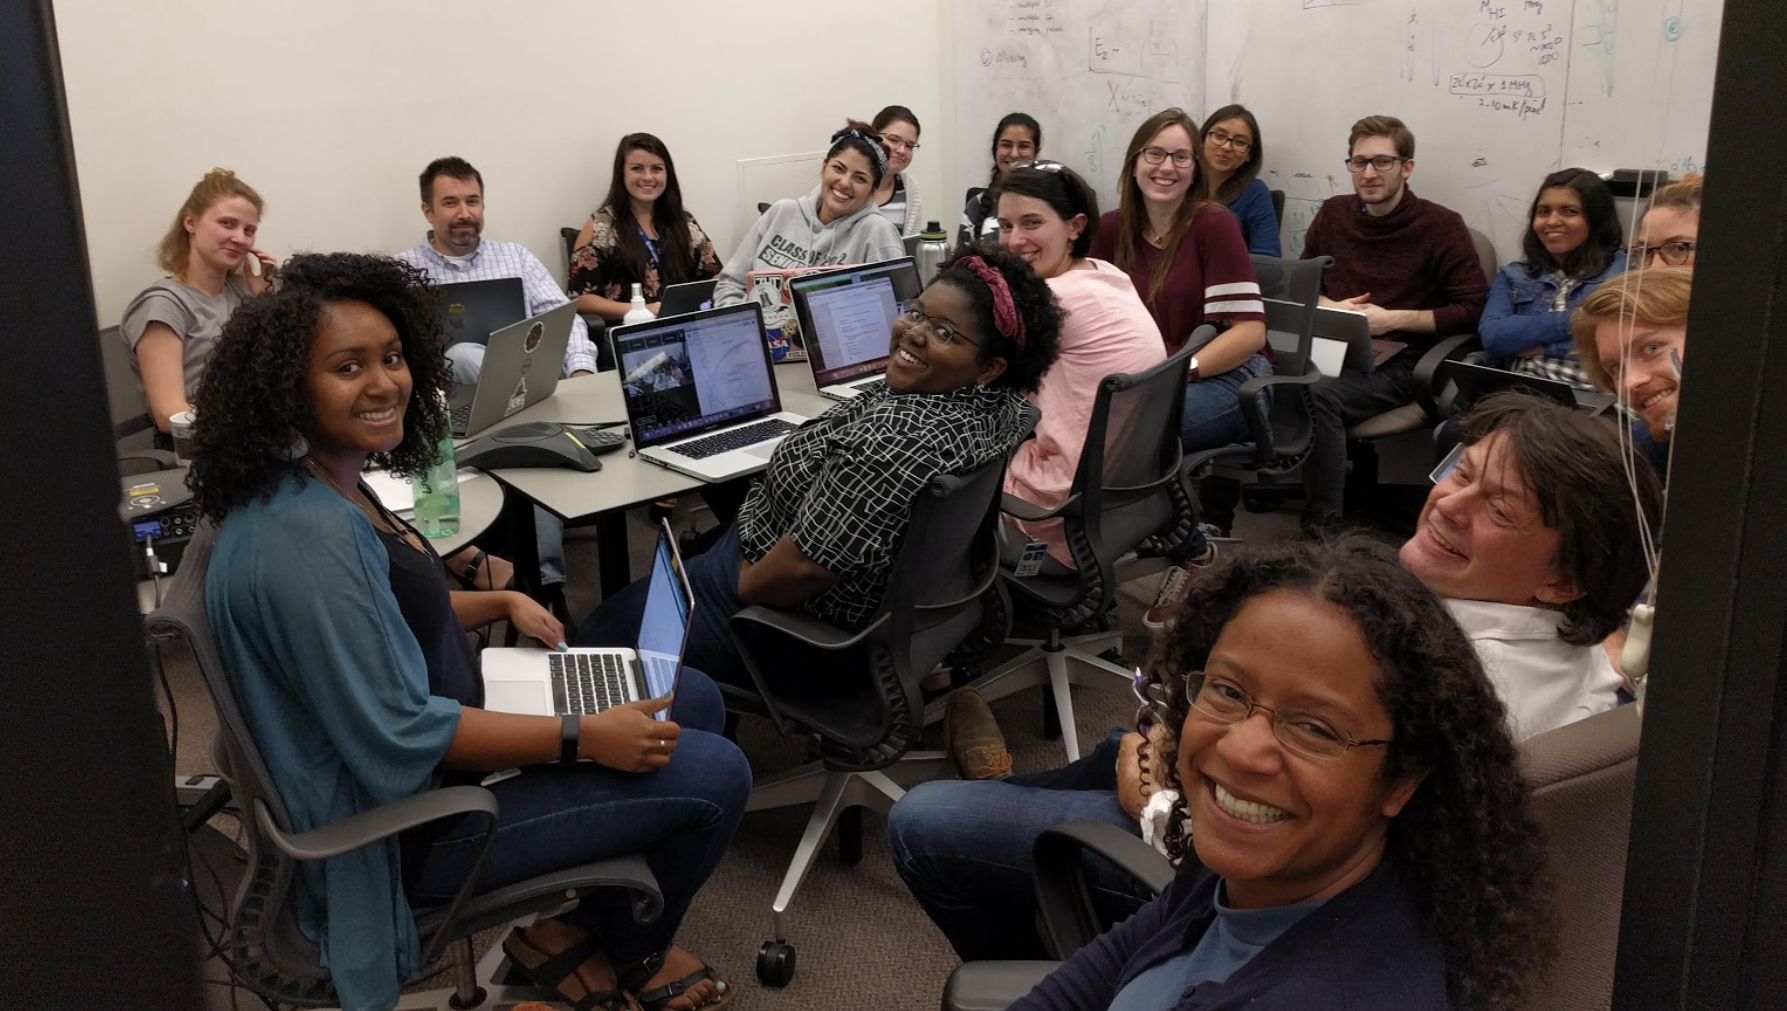
\includegraphics[width=0.66\textwidth]{interns.png}
  \caption*{The summer 2018 intern group at Fermilab's 7th floor, with the 
three senior scientist mentors, our postdoc, and one high school student. 
Three of five of the LSSTC funded interns are present.}
\end{figure}

\newpage
\section{The implementation of this program}

Fermilab has an active internship program. Two internship programs
have been mentioned, and there are four others. The internship
programs here share a Summer Undergraduate Lecture Series by
Lab and visiting scientists. There is an end of summer poster
session given by the summer interns. All of these interns
are housed near the Lab, some on the Lab; we have institutional
experience in handling housing. Lastly, as the US center for
experimental high energy physics, Fermilab itself inspires
the imagination of its interns: they are working at the frontier
of knowledge.

Our base summer intern selection process is to attract
University of Chicago Physics and Astronomy undergraduates.
The Lab has many scientists on joint appointments with
the University of Chicago. When at the University they find
that there are  many more students
requesting research projects then there is the possibility of
the University to support- we believe this is an opportunity.
Other avenues exist: our User community has many undergraduates
from which we could make invitations, 
and the Lab performs student selection for many of its summer
intern programs.

We have identified the right post-baccalaureate candidate:



